\documentclass[10pt]{beamer}

\usepackage{amsmath}
\usepackage{graphicx}


\title{Exercise 11}
\author{Shujun Wang}
\institute{University of Zurich}
\date{November, 2021}

\setbeamertemplate{caption}[numbered]

\begin{document}

\frame{\titlepage}

\begin{frame}
\frametitle{Title 1}
\framesubtitle{Equation}
Equation 1:
\begin{equation}
a^2 + b^2 = c^2
\end{equation}
Equation 2:
\begin{equation}
\frac{1+ 2x}{3 + 2y}
\end{equation}
\end{frame}

\begin{frame}
\frametitle{Title 2}
\framesubtitle{Theorem}
\begin{theorem}
Let \(f\) be a function whose derivative exists in every point, then \(f\) is a continuous function.
\end{theorem}
\end{frame}

\begin{frame}
\frametitle{Title 3}
\framesubtitle{Figure}
\begin{figure}
\centering
\begin{minipage}[b]{0.4\textwidth}
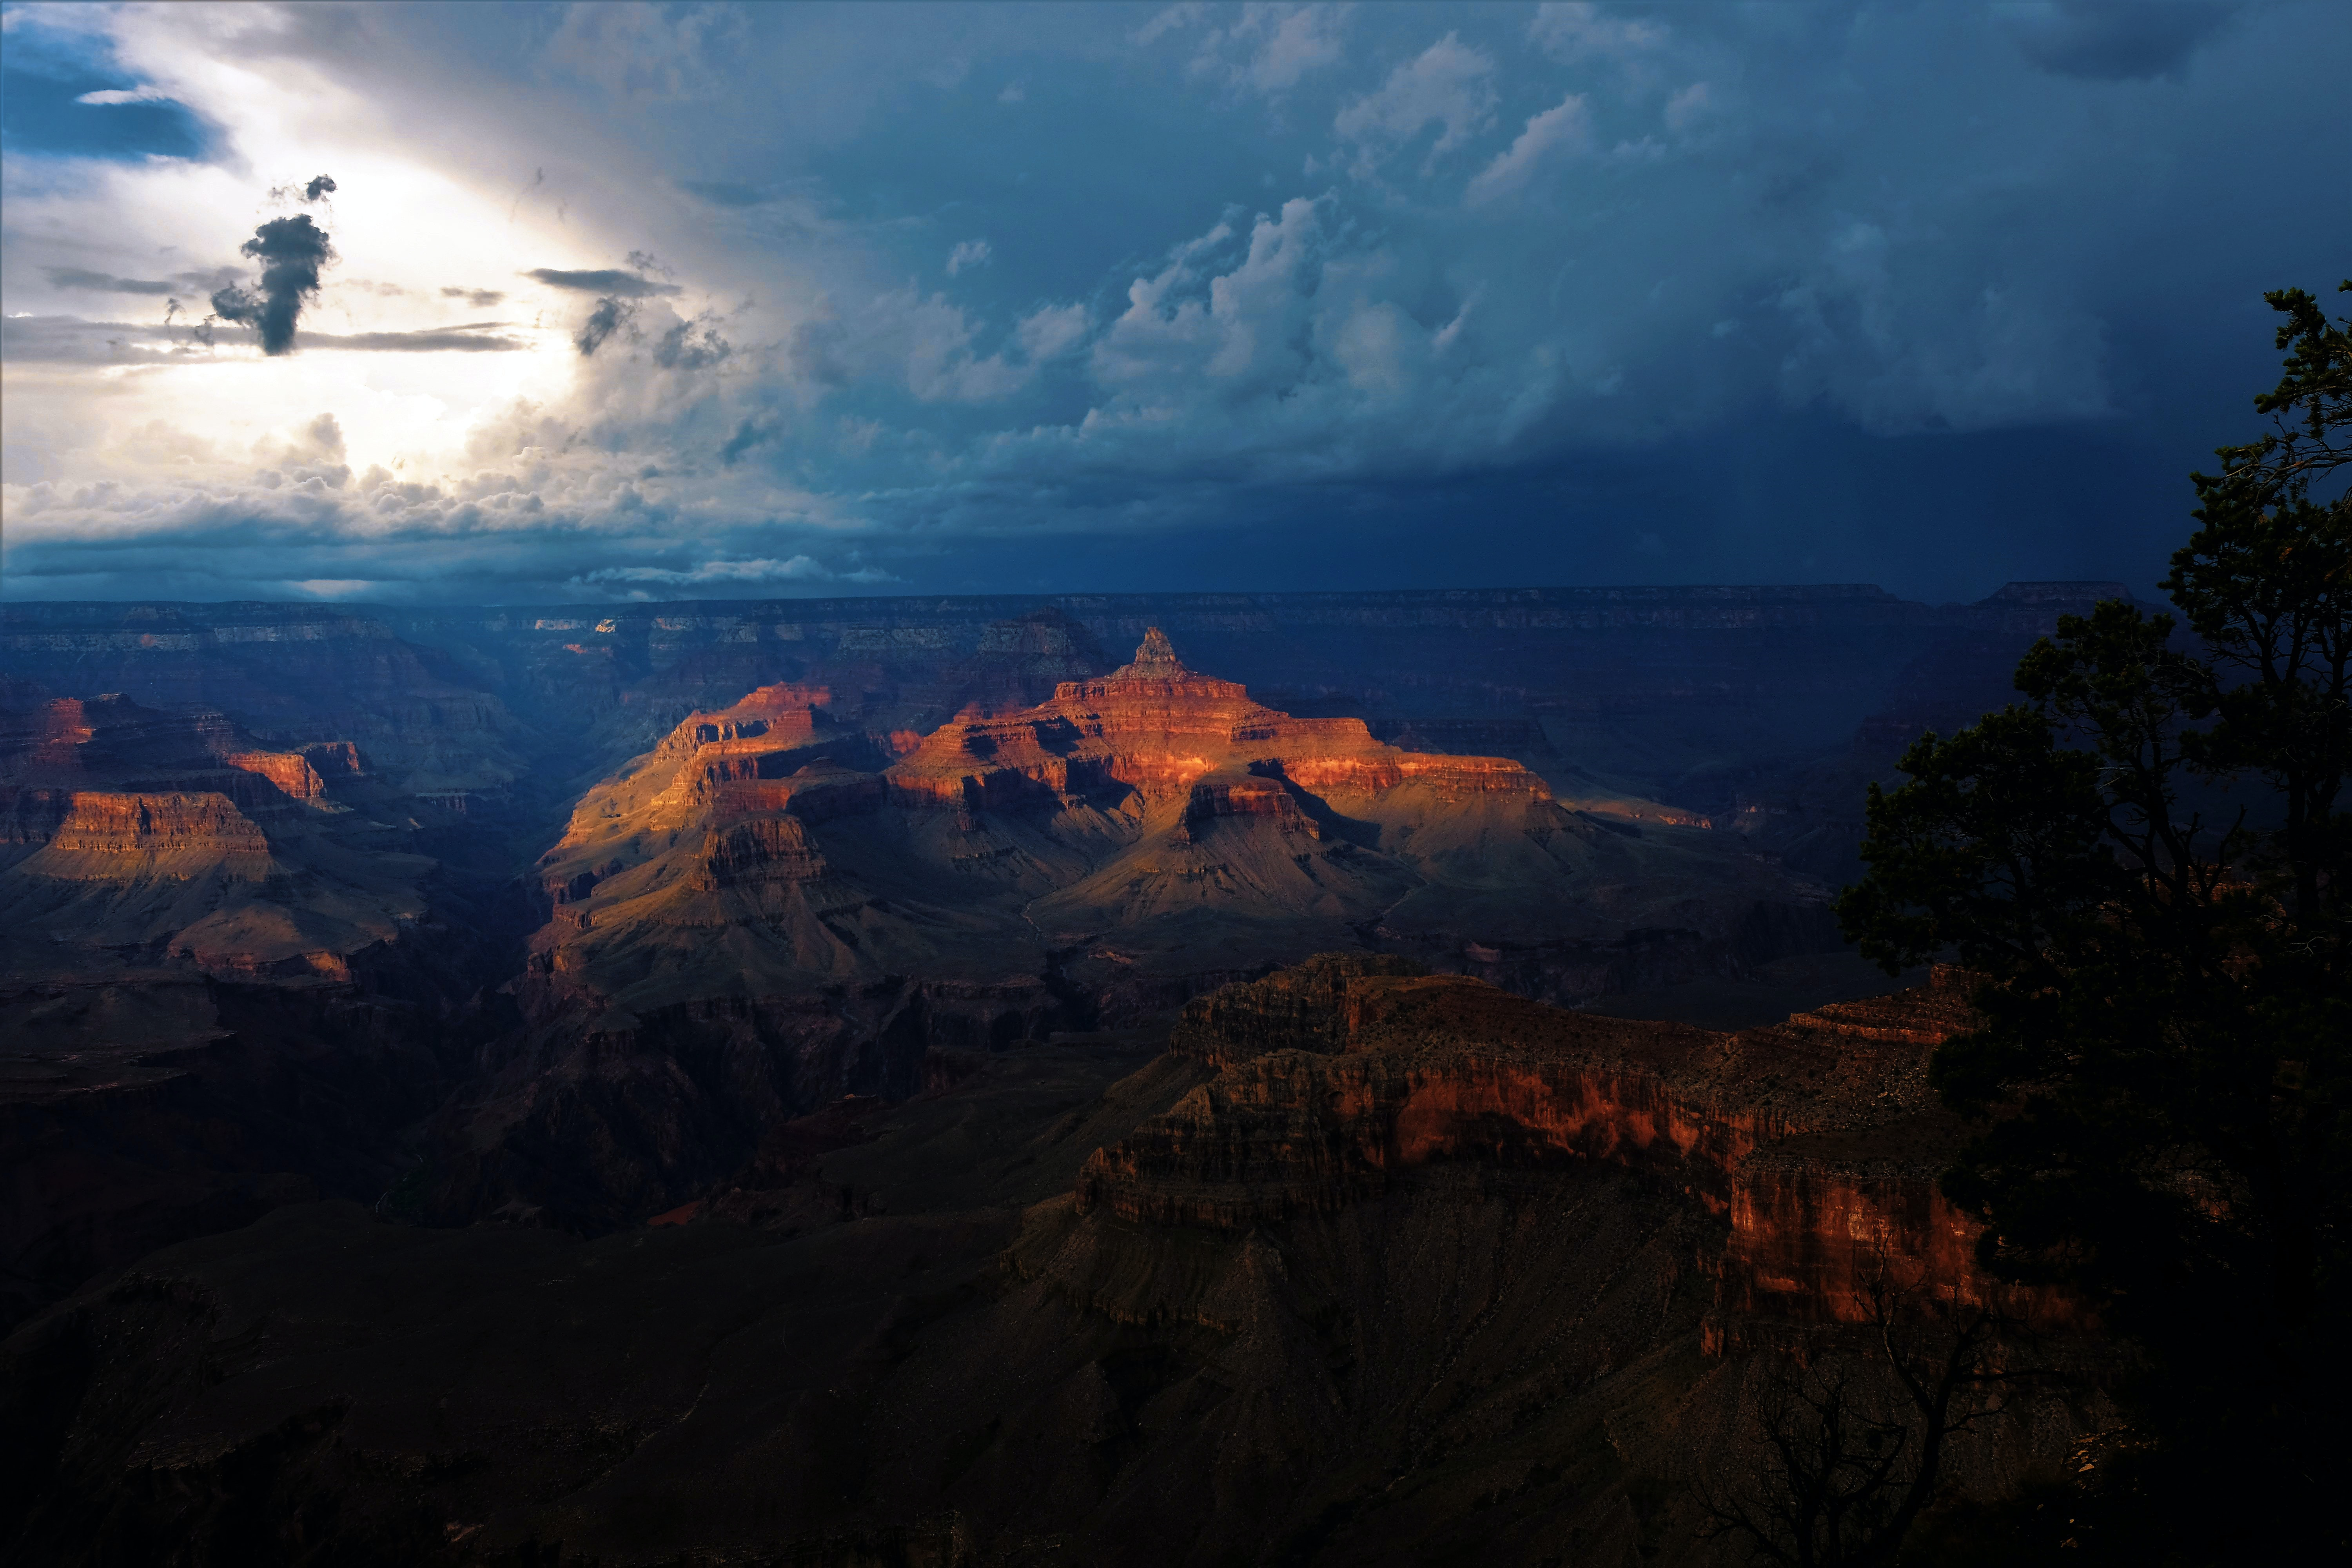
\includegraphics[width=\linewidth]{figure1.jpg}
\caption{Beautiful}
\end{minipage}
\begin{minipage}[b]{0.4\textwidth}
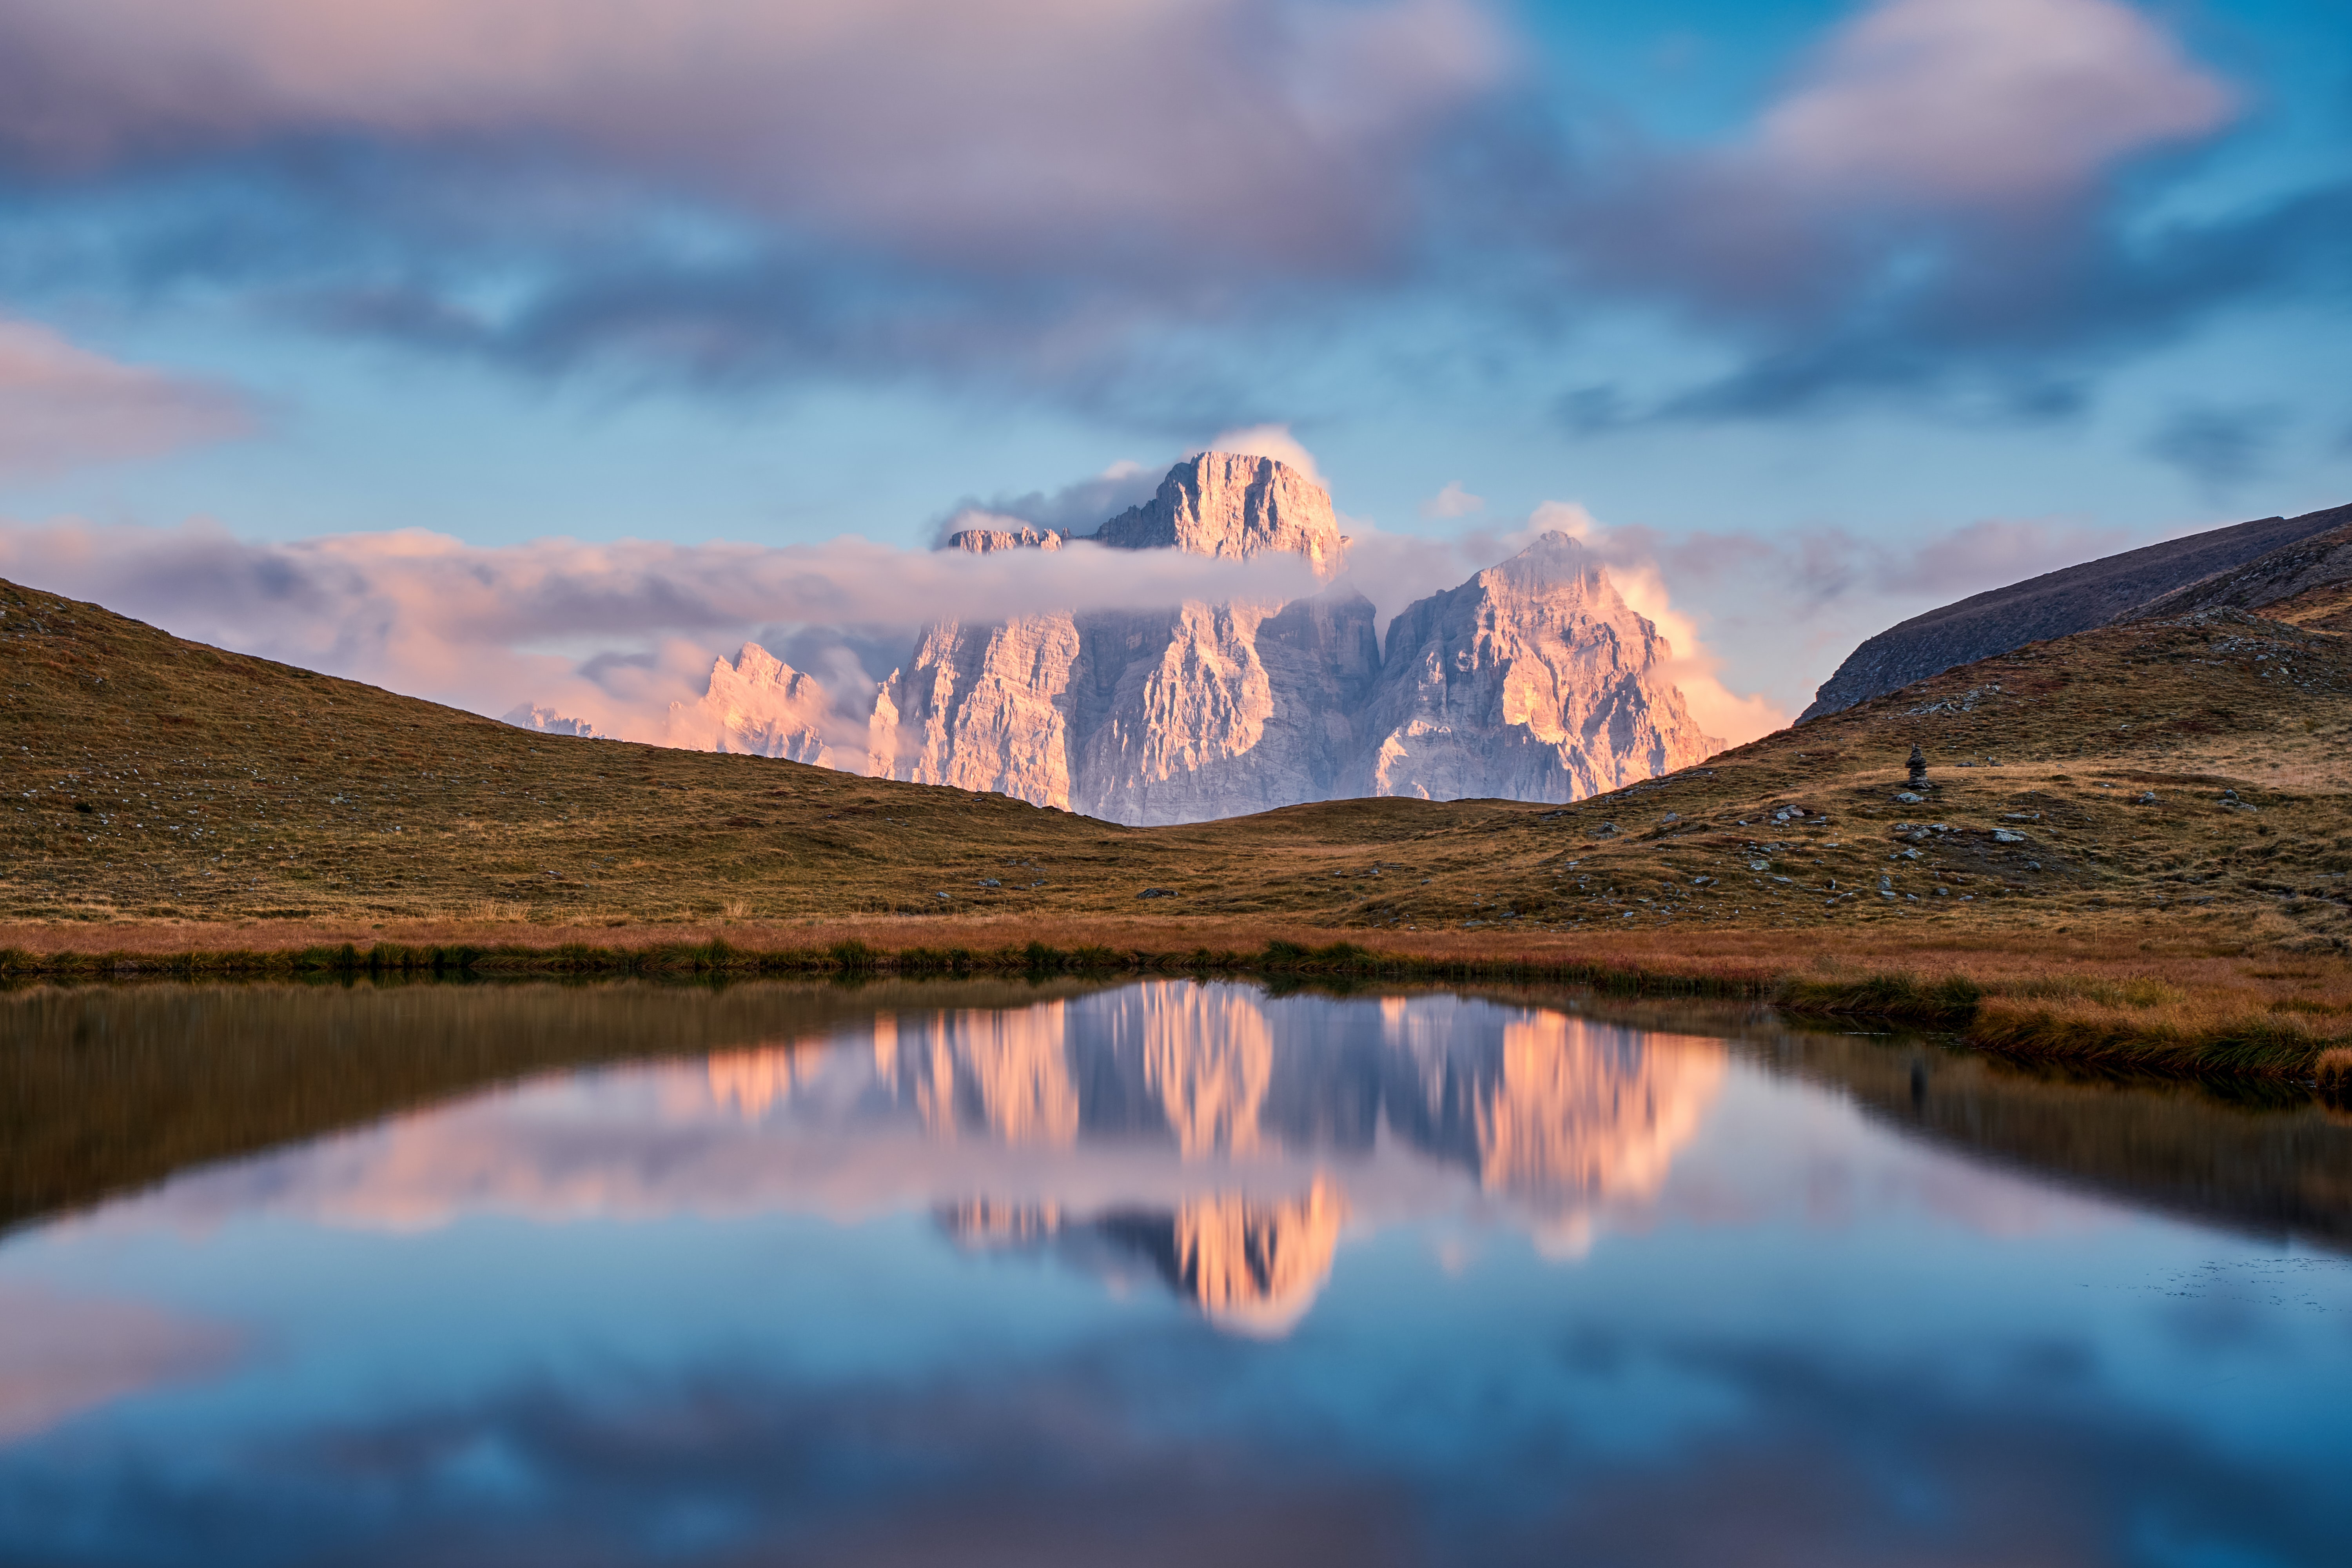
\includegraphics[width=\linewidth]{figure2.jpg}
\caption{Scenery}
\end{minipage}
\end{figure}
\end{frame}


\end{document}